% !TEX root = ../00_thesis.tex

%-------------------------------------------------------------------------------
\section{Overview of \triscale}
\label{sec:triscale_overview}
%-------------------------------------------------------------------------------

This section provides a high-level description of \triscale.
First, we illustrate how \triscale clarifies the interpretation of the results of networking experiments with a concrete example~(\cref{subsec:triscale_intro_example}),
then we present the core principles of \triscale and introduce the structure of the framework~(\cref{subsec:triscale_overview}).

\afterpage{
\begin{landscape}
  \begin{figure}
    \centering
    \begin{subfigure}[t]{0.48\linewidth}
        \centering
       	\href{\triscalefig{Figure-1a}}{
        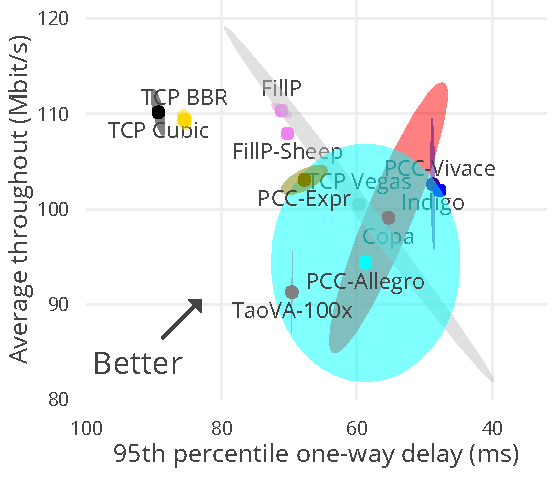
\includegraphics[scale=1]{Figures/plot_zoom_pantheon}}

        \caption{Data analysis and visualization reproduced from~\cite{yan18pantheon}. The dots represent the mean performance of the runs; the ellipses represent the $(1-\sigma)$ variation across runs.}
        \label{fig:example_pantheon}
    \end{subfigure}%
    \hfill
    \begin{subfigure}[t]{0.48\linewidth}
        \centering
        \href{\triscalefig{Figure-1b}}{
        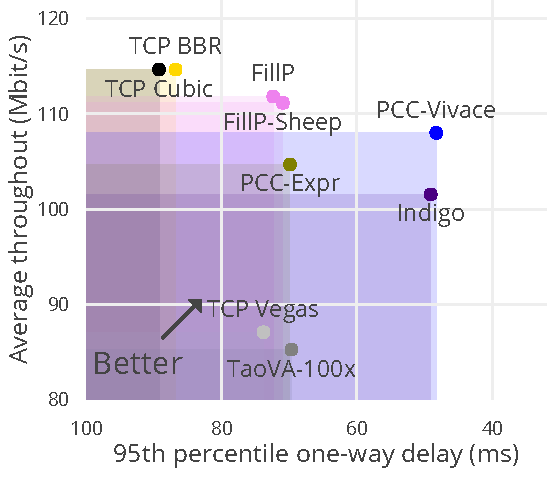
\includegraphics[scale=1]{Figures/plot_zoom_triscale}}

        \caption{Data analysis and visualization produced by \triscale. The dots represent the KPIs of each scheme. Shaded areas represent dominance regions: \emph{scheme~$A$} performs better than \emph{scheme~$B$} if the KPI of~$B$ lies in the dominance region of~$A$.}
        \label{fig:example_triscale}
    \end{subfigure}
    \caption{%
    The same data may be analyzed in different ways. \Cref{fig:example_triscale} illustrates the output of a data analysis performed by \triscale. Compared with \Cref{fig:example_pantheon}, the interpretation of the results is more intuitive: The performance of each scheme is reduced to a single point (\triscale's KPIs), which makes the comparison between the schemes unambiguous.
    \triscale's KPIs are not arbitrary: they are robust statistics estimating, with a given confidence level, the expected performance if the experiment was repeated (see~\cref{subsec:KPIs}). As such, the KPIs inherently account for the variability in the results.
    \capt{Experiment settings: 1 flow, 10 runs, 30\s runtime, emulated network (sample data from the congestion-control case study~\cref{sec:triscale_eval}).}}
    \label{fig:example_pantheon_triscale}
  \end{figure}
\end{landscape}
}


%-------------------------------------------------------------------------------
\subsection{Shortcomings in the Data Analysis}
\label{subsec:triscale_intro_example}

Let us assume you are a networking researcher discovering the field of congestion control and trying to understand the strengths and weaknesses of the state-of-the-art.
Luckily, the community has developed useful tools such as Pantheon~\cite{yan18pantheon}, a data collection framework that facilitates comparisons between different schemes.

You are especially interested in comparing the average throughput and one-way delay of long-running full-throttle flows, \ie stable flows whose only throttling/limiting factor is the congestion control.
You start with one flow and evaluate performance using the MahiMahi~\cite{netravali2015mahimahi} emulator (integrated in Pantheon), following the same settings as in the original paper~\cite{yan18pantheon}, \ie~10~runs of 30~seconds each. You collect data for the 17 schemes available at the time of your experiment.

Pantheon focuses on collecting data, not on their interpretation. Yet, the interpretation is not trivial. Consider for example the data shown in \Cref{fig:example_pantheon} (reproduced from~\cite{yan18pantheon}). Multiple questions arise:

\begin{itemize}

    % Hard to compare
    \item
    Can the schemes be compared?
    It appears that \textit{Vegas} performs better than \eg \textit{TaoVA-100x}.
    However, the ellipses capture the variability of results across multiple runs: more precisely, they represent the $(1-\sigma)$ variation across runs.
    What can you then conclude about the actual performance of these schemes?
    Can you conclude anything when ellipses are overlapping?
    For example, can you say that \textit{Vegas} performs better than \textit{PCC-Expr}?

    % Confidence? Are results trustworthy?
    \item
    What is the confidence in the comparison? Intuitively, the results of \eg \textit{PCC-Allegro}, which has a large variability, are ``less trustworthy'' than \eg \textit{FillP-Sheep}, for which you cannot even see the ellipse on the graph. But can you quantify the confidence in the result?

    % Impact of the runtime on the results?
    \item
    Is a runtime of 30~seconds (the default setting) really long enough to capture the long-running performance of the various schemes?

    % Are the results reproducible?
\end{itemize}

These questions relate to the \feature{Robustness} and \feature{Rationality} requirements mentioned in~\cref{sec:triscale_intro}.
The data analysis shown in \Cref{fig:example_pantheon} leaves these questions unanswered.
Worse, the analysis may suggest wrong interpretations: the ellipses are a two-dimensional representation of the standard deviation across the runs, which suggests that one expects about 68\% of the data points to fall in that region.
However, this is correct \textbf{only if} the underlying distribution is normal, which is hardly ever true (\cref{sec:stats}).

Let us now compare the \emph{same raw data}, but analyzed using \triscale (\Cref{fig:example_triscale}).
The points in the plot represent \triscale's Key Performance Indicators (KPIs).
A KPI is defined as the estimate of a given percentile of one performance metric distribution.
For example: with 10 runs, we collect 10 samples of the performance metric ``average throughput''.
Based on these 10~samples, we can \emph{estimate} some properties of the underlying distribution of ``average throughput'' (\ie the \emph{unknown} distribution one would obtain with infinitely many samples).
\triscale's KPIs estimate percentiles of that underlying distribution with a certain confidence.
In \Cref{fig:example_triscale}, the ``average throughput'' KPI is defined as the estimate of the 25th percentile with a 75\% confidence level; in other words, the KPI has a 75\% probability to correctly estimate the 25th percentile of the distribution (more details in \cref{subsec:KPIs}).

Since KPIs are individual points, they unambiguously compare different schemes.
\triscale shows, for example, that \textit{Vegas} is not generally better than \textit{TaoVA-100x}: each performs better in either delay or throughput (\Cref{fig:example_triscale}).
Furthermore, \textit{PCC-Expr} performs strictly better than \textit{Vegas}, whereas \Cref{fig:example_pantheon} suggests the opposite.
The KPIs in \Cref{fig:example_triscale} can be interpreted as follows:\emph{
with a 75\% probability, 75\% of the runs will yield a performance at least as good as the KPI value} (\ie higher throughput and lower delay).

Observe that \textit{Copa} and \textit{PCC-Allegro} are no longer present in \Cref{fig:example_triscale}.
Indeed, \triscale first verifies whether the schemes have ``converged''; that is, it checks whether the performance metrics have reached stable values (\cref{subsec:test_convergence}).
These two schemes eventually converge, but it often takes more than 30 seconds.
In \Cref{fig:example_triscale},
\emph{the KPIs are representative of the ``long-running'' performance} (\ie the performance expected if the scheme would run ``forever'') with a 95\% probability.

\fakepar{Conclusion} 
Tools like Pantheon~\cite{yan18pantheon} support data collection, but leave to the researcher to design the experiments and analyze the data, leading to ambiguous interpretations and non-reproducible results.
\triscale aims to fill this gap.
\afterpage{
\begin{landscape}
  \begin{figure}
  	\centering
  	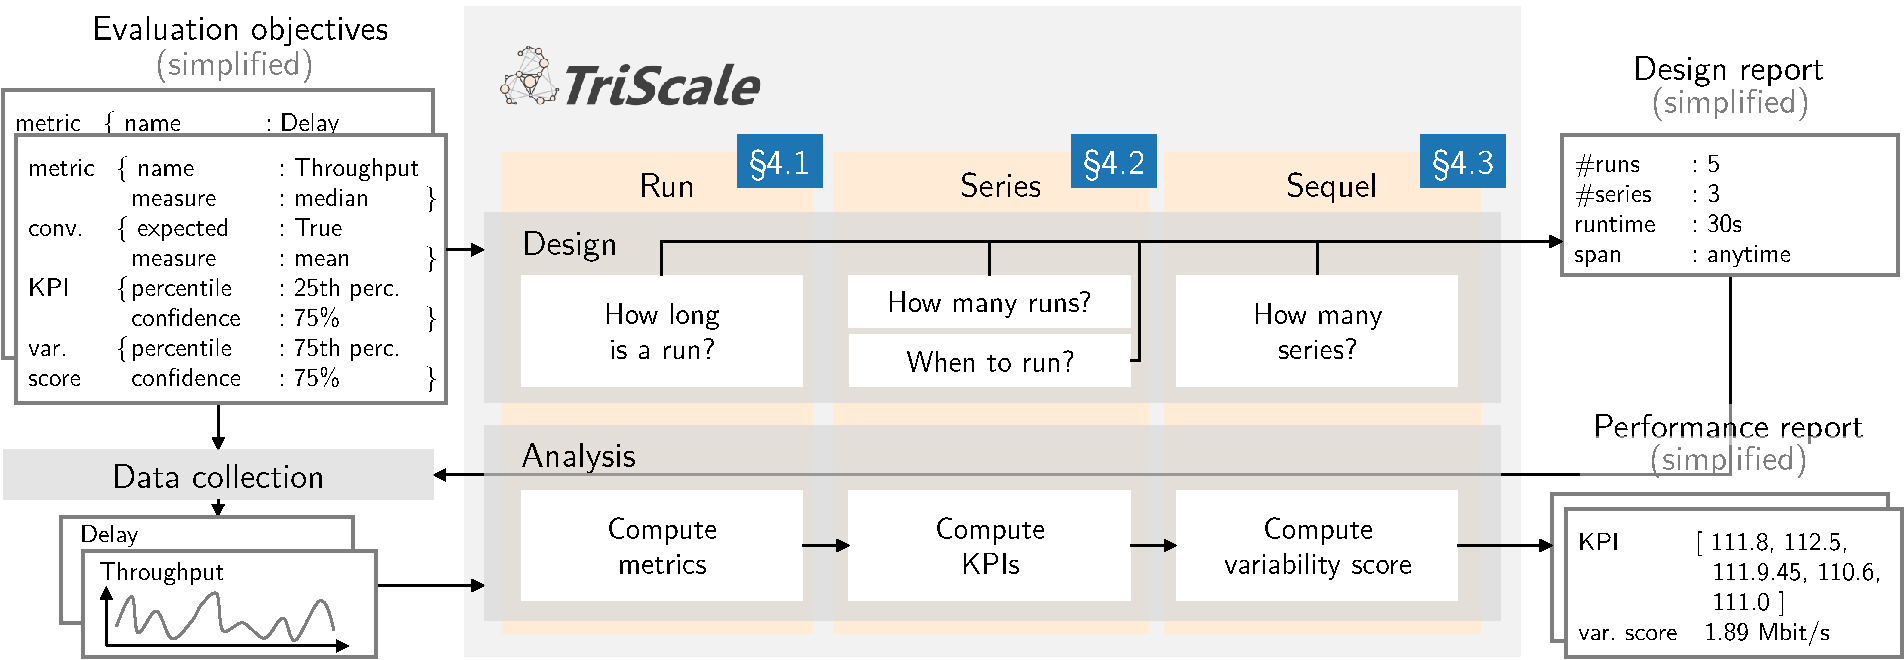
\includegraphics[width=0.955\linewidth]{triscale_overview_flat}
  	\caption{Overview of \triscale.
  		\capt{\triscale is a framework supporting the design and data analysis of networking experiments.
  		\triscale assists the user in the design phase with a systematic methodology to answer important experiment design questions such as ``How many runs?'' and  ``How long should the runs be?''. After the data has been collected, \triscale supports the user by automating the data analysis. The framework implements robust statistics that handle the intrinsic variability of experimental networking data and return expressive performance reports as well as a variability score.
  		}
  		}
  	\label{fig:overview}
  \end{figure}
\end{landscape}
}


%-------------------------------------------------------------------------------
\subsection{Methodological Core Principles}
\label{subsec:triscale_overview}

We now introduce how \triscale supports the design and analysis of networking experiments. The structure and inputs/outputs of the \triscale framework are illustrated in \Cref{fig:overview}.

\fakepar{Experiment design}
\triscale achieves \feature{Rationality}~(\cref{sec:triscale_intro}) by formalizing the evaluation definition and by streamlining the design of experiments.
The design phase starts with the definition of the evaluation objectives: for each performance dimension, the user defines the metric, the convergence requirements, a KPI, and a variability score.
From these inputs, \triscale returns the minimal number of runs (\emph{\#runs}) and \mbox{series} (\emph{\#series}) necessary to compute the chosen KPIs and variability scores; that is, \emph{how many runs to perform}.
Using the data from a few test runs, \triscale can assess whether the length of a run (the \emph{runtime}) is suitable; \ie \emph{how long a run should be}.
Finally, \triscale uses network profiling information to avoid time-dependent bias in the experiments; \ie it tells \emph{when the experiment should be carried out} (the \emph{span}).

In the congestion-control example presented previously, the evaluation objectives are the following.
The metrics' measures for throughput and delay are the median and 95th percentile, respectively.
The KPIs are chosen as the 25th and 75th percentiles with 75\% confidence, for which \triscale returns a minimum of 5 runs.
Convergence is expected and initial tests reveal that \textit{PCC-Allegro} and \textit{Copa} almost never converge within 30\s~(see \cref{sec:triscale_eval}).
As experiments are carried out in emulation, there is no time dependency and therefore it does not matter when the experiment is performed~(\ie \emph{span: anytime}).


\fakepar{Data analysis}
\triscale achieves \feature{Robustness} (\cref{sec:triscale_intro}) by
applying carefully-chosen statistical methods, verifying that their hypotheses hold for the collected data, and automating the computations.
In particular, once the experiment has been designed and the data collected, the raw data is passed to \triscale for analysis.
The analysis is divided into three timescales: \emph{runs}, \emph{series}, and \emph{sequels} (hence the name of \triscale):\\
  A \textbf{run} is one execution of the evaluation scenario (\eg a 30\s execution of one congestion-control scheme).
  The raw data from one run are analyzed to compute the performance metrics defined in the evaluation objectives.
  This timescale leads to one number per run and per metric~(\cref{subsec:metrics}).\\
  %
  % \item[Series]
  A \textbf{series} is a set of runs performed closely in time (\eg in the same day).
  Multiple runs allow to account for the inherent variability in the experiments.
  This timescale leads to one number per series and per metric, \ie \triscale's KPIs~(\cref{subsec:KPIs}).\\
  %
  % \item[Sequels]
  A \textbf{sequel} is a repetition of a series, performed at a later point in time (\eg a week, a month, or a year later).
  \triscale uses sequels (\ie a set of series) to compute a variability score which captures the long-term variability of the KPIs.
  This timescale leads to one number per metric (\cref{subsec:repeatability}).
%
% \end{description}

In the previous example, \triscale returns a pair of KPIs per scheme, which allow to unambiguous compare the different schemes with a quantified confidence (in this case, 75\% -- see \cref{fig:example_triscale}).
